\documentclass[12pt,a4paper]{report}


\usepackage[utf8]{inputenc}
\usepackage[romanian]{babel}
\usepackage[T1]{fontenc}
\usepackage{lmodern} 
\usepackage{microtype} 
\usepackage{xcolor} 
\usepackage{titlesec} 
\usepackage{tcolorbox} 
\usepackage{booktabs} 
\usepackage{tabularx} 
\usepackage{listings} 
\usepackage{setspace} 
\usepackage{fancyhdr} 
\usepackage[hidelinks]{hyperref} 
\usepackage{geometry} 

\usepackage{tikz}
\usepackage{pgfgantt} 
\usepackage{pgfplots}
\usepackage{amsmath}
\usepackage{amssymb}
\pgfplotsset{compat=1.18}
\usetikzlibrary{positioning, arrows, shapes, shadows, trees, mindmap, backgrounds, calc, fit, decorations, decorations.pathreplacing, calligraphy, matrix, arrows.meta}


\geometry{
  a4paper,
  top=2.5cm,
  bottom=2.5cm,
  left=2.5cm,
  right=2.5cm
}


\pagestyle{fancy}
\fancyhf{}
\renewcommand{\headrulewidth}{0.5pt}
\renewcommand{\footrulewidth}{0.5pt}
\fancyhead[L]{Utilitar AI pentru Analiza Criptografica}
\fancyhead[R]{\thepage}
\fancyfoot[C]{Lucrare de Licenta}


\onehalfspacing


\titleformat{\chapter}[display]
{\normalfont\huge\bfseries\color{blue!70!black}}
{\chaptertitlename\ \thechapter}{20pt}{\Huge}
\titlespacing*{\chapter}{0pt}{50pt}{40pt}

\titleformat{\section}
{\normalfont\Large\bfseries\color{blue!60!black}}
{\thesection}{1em}{}
\titlespacing*{\section}{0pt}{3.5ex plus 1ex minus .2ex}{2.3ex plus .2ex}

\titleformat{\subsection}
{\normalfont\large\bfseries\color{blue!50!black}}
{\thesubsection}{1em}{}


\lstset{
  basicstyle=\ttfamily\small,
  breaklines=true,
  commentstyle=\color{green!60!black},
  keywordstyle=\color{blue},
  stringstyle=\color{red},
  numbers=left,
  numberstyle=\tiny\color{gray},
  frame=single,
  framesep=5pt,
  framexleftmargin=5pt,
  tabsize=4,
  captionpos=b,
  showstringspaces=false,
  backgroundcolor=\color{gray!10}
}
\definecolor{infobox}{RGB}{230, 240, 255}
\definecolor{notebox}{RGB}{255, 240, 230}
\begin{document}
\begin{titlepage}
  \centering
  \vspace*{2cm} % Increased top spacing for a grander feel
  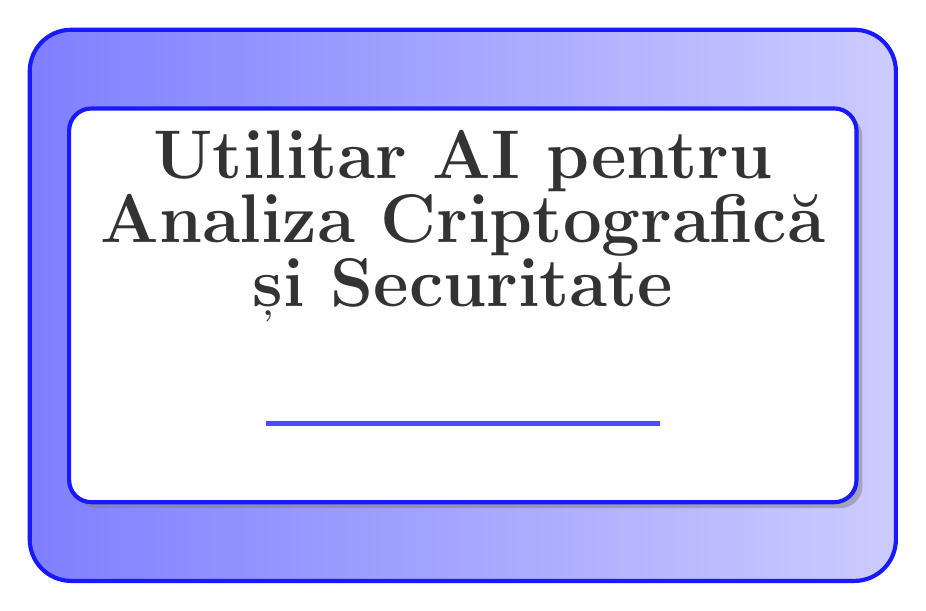
\begin{tikzpicture}
      \shade[left color=blue!50, right color=blue!20, draw=blue!90, line width=1.5pt, rounded corners=15pt] 
          (-1,-1) rectangle (10,6); % Enlarged dimensions
      \filldraw[fill=white, draw=blue!90, line width=1.5pt, rounded corners=8pt, drop shadow={opacity=0.5, color=gray}] 
          (-0.5,0) rectangle (9.5,5); % Slightly larger with shadow for depth
      \node[align=center, font=\fontsize{24}{18}\selectfont\bfseries, text=black!80] at (4.5,3.5) 
          {Utilitar AI pentru \\ Analiza Criptografică \\ și Securitate};
      \draw[blue!70, line width=2pt, rounded corners=2pt] (2,1) -- (7,1);
  \end{tikzpicture}
  \vspace{2cm} % Increased bottom spacing for balance
\end{titlepage}
\tableofcontents
\thispagestyle{empty}
\clearpage

\chapter{Introducere si Prezentare Generala}

\section{Contextul Proiectului}
Proiectul propune dezvoltarea unui sistem integrat care combina
inteligenta artificiala cu diverse tehnici criptografice pentru
a oferi o platforma completa de analiza a criptogramelor,
criptare/decriptare, analiza a teoriei numerelor si evaluare a
securitatii parolelor. Intr-o era in care securitatea informatiilor
devine din ce in ce mai importanta, acest sistem va servi ca
instrument educational si practic pentru studenti, cercetatori si
profesionisti in domeniul securitatii informatice.

\section{Obiective}
\begin{itemize}
  \item Crearea unei platforme integrate pentru analiza criptografica
  \item Implementarea unui motor de conversatie bazat pe LLM specializat in criptografie
  \item Dezvoltarea modulelor de analiza si atac pentru diverse algoritmi criptografici
  \item Integrarea bazelor de date pentru numere prime si semiprime
  \item Implementarea algoritmilor post-quantum
  \item Asigurarea scalabilitatii si securitatii sistemului
\end{itemize}

\section{Valoare Academica si Practica}
Lucrarea aduce contributii semnificative prin:
\begin{itemize}
  \item Integrarea tehnicilor de ML/DL in analiza criptografica
  \item Abordarea unitara a mai multor aspecte ale criptografiei
  \item Implementarea practica a algoritmilor post-quantum
  \item Crearea unei interfete conversationale pentru rezolvarea problemelor criptografice
\end{itemize}

\chapter{Arhitectura Sistemului}

\section{Arhitectura Generala}


\begin{figure}[h]
  \centering
  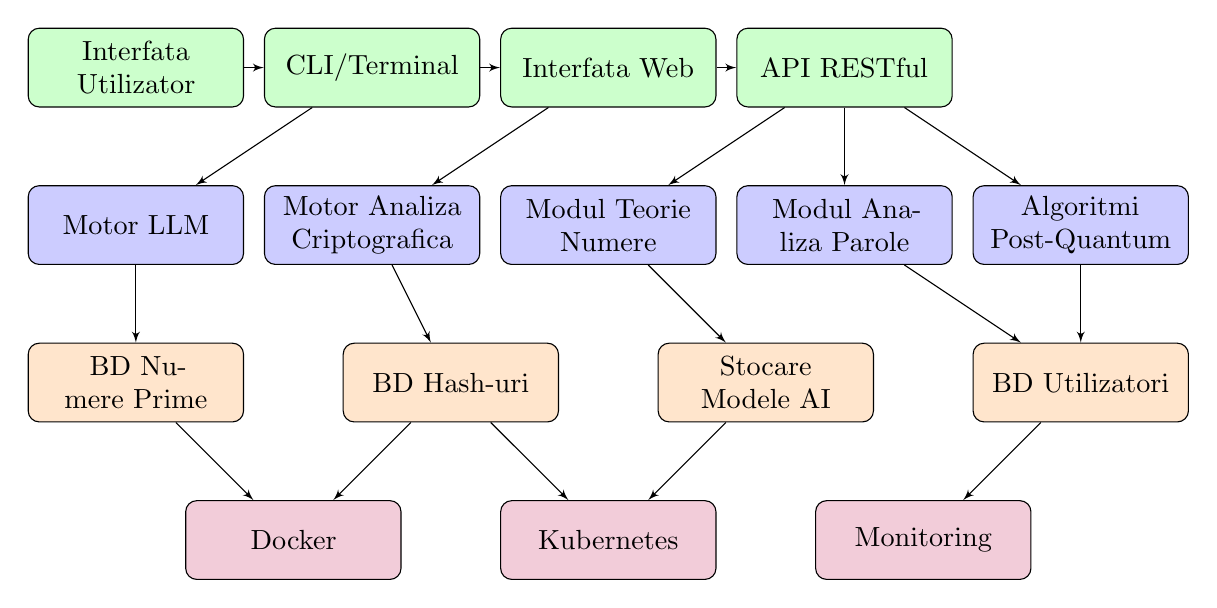
\begin{tikzpicture}[
    auto,
    block/.style={rectangle, draw, fill=blue!20, text width=2.5cm, text centered, minimum height=1cm, rounded corners},
    line/.style={draw, -latex'},
    cloud/.style={draw, ellipse, fill=red!20, text width=2.5cm, text centered, minimum height=1cm}
    ]
    
    
    \node[block, fill=green!20] (ui) at (0,8) {Interfata Utilizator};
    \node[block, fill=green!20] (cli) at (3,8) {CLI/Terminal};
    \node[block, fill=green!20] (web) at (6,8) {Interfata Web};
    \node[block, fill=green!20] (api) at (9,8) {API RESTful};
    
    
    \node[block, fill=blue!20] (llm) at (0,6) {Motor LLM};
    \node[block, fill=blue!20] (crypto) at (3,6) {Motor Analiza Criptografica};
    \node[block, fill=blue!20] (numth) at (6,6) {Modul Teorie Numere};
    \node[block, fill=blue!20] (passwd) at (9,6) {Modul Analiza Parole};
    \node[block, fill=blue!20] (pqc) at (12,6) {Algoritmi Post-Quantum};
    
    
    \node[block, fill=orange!20] (prime) at (0,4) {BD Numere Prime};
    \node[block, fill=orange!20] (hash) at (4,4) {BD Hash-uri};
    \node[block, fill=orange!20] (ai) at (8,4) {Stocare Modele AI};
    \node[block, fill=orange!20] (user) at (12,4) {BD Utilizatori};
    
    
    \node[block, fill=purple!20] (docker) at (2,2) {Docker};
    \node[block, fill=purple!20] (k8s) at (6,2) {Kubernetes};
    \node[block, fill=purple!20] (monitor) at (10,2) {Monitoring};
    
    
    \draw[line] (ui) -- (cli);
    \draw[line] (cli) -- (web);
    \draw[line] (web) -- (api);
    
    \draw[line] (cli) -- (llm);
    \draw[line] (web) -- (crypto);
    \draw[line] (api) -- (numth);
    \draw[line] (api) -- (passwd);
    \draw[line] (api) -- (pqc);
    
    \draw[line] (llm) -- (prime);
    \draw[line] (crypto) -- (hash);
    \draw[line] (numth) -- (ai);
    \draw[line] (passwd) -- (user);
    \draw[line] (pqc) -- (user);
    
    \draw[line] (prime) -- (docker);
    \draw[line] (hash) -- (docker);
    \draw[line] (hash) -- (k8s);
    \draw[line] (ai) -- (k8s);
    \draw[line] (user) -- (monitor);
    
  \end{tikzpicture}
  \caption{Arhitectura generala a sistemului}
  \label{fig:arhitectura}
\end{figure}

\section{Componente Principale}

\subsection{Frontend}
\begin{itemize}
  \item \textbf{Interfata CLI/Terminal}: Interactiune directa prin comanda
  \item \textbf{Interfata Web}: Acces prin browser cu suport pentru diverse dispozitive
  \item \textbf{API RESTful}: Endpointuri pentru servicii si integrare cu alte sisteme
\end{itemize}

\subsection{Backend}
\begin{itemize}
  \item \textbf{Motor LLM}: Procesare in limbaj natural si generare de raspunsuri
  \item \textbf{Motor de Analiza Criptografica}: Modulul central pentru analiza si atacarea criptogramelor
  \item \textbf{Modul Teorie Numere}: Gestionarea operatiilor cu numere prime, factorizare
  \item \textbf{Modul Analiza Parole}: Evaluarea securitatii parolelor si generarea de recomandari
  \item \textbf{Modul Algoritmi Post-Quantum}: Implementarea si testarea algoritmilor rezistenti la atacuri cuantice
\end{itemize}

\subsection{Stocare}
\begin{itemize}
  \item \textbf{Baza de Date Numere Prime/Semiprime}: Cache si acces rapid la informatii despre numere prime
  \item \textbf{Baza de Date Hash-uri}: Pentru verificarea parolelor si hash-urilor cunoscute
  \item \textbf{Stocare Modele AI}: Pentru modelele LLM antrenate si ponderile acestora
  \item \textbf{Baza de Date Utilizatori}: Gestionarea conturilor, preferintelor si istoricului conversatiilor
\end{itemize}

\chapter{Stack Tehnologic}

\section{Stack Tehnologic Detaliat}

\subsection{Backend}
\begin{itemize}
  \item \textbf{Python 3.10+}: Limbaj principal pentru dezvoltarea backend-ului
  \item \textbf{FastAPI}: Framework modern, rapid si asincron pentru API-uri
  \item \textbf{C/C++}: Pentru componente critice de performanta (algoritmi criptografici)
  \item \textbf{Rust}: Pentru module de securitate si performanta ridicata
  \item \textbf{gRPC}: Pentru comunicare eficienta intre microservicii
\end{itemize}

\subsection{Inteligenta Artificiala}
\begin{itemize}
  \item \textbf{PyTorch}: Framework principal pentru antrenarea modelelor LLM
  \item \textbf{TensorFlow/Keras}: Pentru anumite componente specifice
  \item \textbf{Hugging Face Transformers}: Pentru utilizarea si fine-tuning-ul modelelor pre-antrenate
  \item \textbf{ONNX Runtime}: Pentru optimizarea inferentei modelelor
\end{itemize}

\subsection{Criptografie}
\begin{itemize}
  \item \textbf{OpenSSL}: Biblioteca standard pentru implementari criptografice
  \item \textbf{Cryptography (Python)}: Pentru operatii criptografice in Python
  \item \textbf{Liboqs}: Pentru implementari post-quantum
  \item \textbf{NTL}: Pentru algoritmi avansati de teorie a numerelor
  \item \textbf{GMP}: Pentru operatii cu numere de precizie arbitrara
\end{itemize}

\subsection{Stocare Date}
\begin{itemize}
  \item \textbf{PostgreSQL}: Baza de date relationala principala
  \item \textbf{Redis}: Pentru caching si sesiuni
  \item \textbf{MongoDB}: Pentru stocare flexibila a istoricului conversatiilor
  \item \textbf{MinIO}: Pentru stocare de tip obiect (modele AI)
\end{itemize}

\subsection{Containerizare si Orchestrare}
\begin{itemize}
  \item \textbf{Docker}: Pentru containerizarea aplicatiilor
  \item \textbf{Docker Compose}: Pentru dezvoltare si testare locala
  \item \textbf{Kubernetes}: Pentru orchestrare in productie
  \item \textbf{Helm}: Pentru gestionarea deployment-urilor Kubernetes
\end{itemize}

\subsection{Securitate}
\begin{itemize}
  \item \textbf{JWT}: Pentru autentificare si autorizare
  \item \textbf{OAuth2}: Pentru integrare cu sisteme externe
  \item \textbf{Keycloak}: Pentru management identitate (optional)
  \item \textbf{Vault}: Pentru gestionarea secretelor
\end{itemize}

\subsection{Frontend}
\begin{itemize}
  \item \textbf{React}: Pentru interfata web
  \item \textbf{NextJS}: Pentru SSR si optimizare
  \item \textbf{TailwindCSS}: Pentru stilizare rapida
  \item \textbf{shadcn/ui}: Pentru componente reutilizabile
\end{itemize}

\subsection{Monitorizare si Logging}
\begin{itemize}
  \item \textbf{Prometheus}: Pentru colectarea metricilor
  \item \textbf{Grafana}: Pentru vizualizarea metricilor
  \item \textbf{ELK Stack}: Pentru logging centralizat
  \item \textbf{Jaeger}: Pentru distributed tracing
\end{itemize}

\section{Justificarea Tehnologiilor}

\subsection{Backend}
\begin{itemize}
  \item \textbf{Python}: Versatil, bogat in biblioteci pentru ML si criptografie, productivitate ridicata
  \item \textbf{FastAPI}: Performanta superioara, documentatie automata, suport asincron
  \item \textbf{C/C++}: Performanta critica pentru algoritmi criptografici intensivi
  \item \textbf{Rust}: Siguranta la nivel de memorie, performanta apropiata de C/C++
\end{itemize}

\subsection{AI si ML}
\begin{itemize}
  \item \textbf{PyTorch}: Flexibilitate, comunitate activa, suport excelent pentru NLP
  \item \textbf{Hugging Face}: Acces la modele pre-antrenate, simplificarea fine-tuning-ului
  \item \textbf{ONNX}: Optimizare pentru inferenta, portabilitate intre framework-uri
\end{itemize}

\subsection{Containerizare}
\begin{itemize}
  \item \textbf{Docker}: Izolare, reproducibilitate, portabilitate
  \item \textbf{Kubernetes}: Scalabilitate, auto-healing, orchestrare avansata
\end{itemize}

\subsection{Securitate}
\begin{itemize}
  \item \textbf{JWT}: Standard pentru tokenuri de autentificare
  \item \textbf{OpenSSL}: Biblioteca matura si testata pentru operatii criptografice
\end{itemize}

\chapter{Implementarea Modulelor}

\section{Motorul LLM Specializat}

\subsection{Structura Modelului}
Se propune utilizarea unui model de tip encoder-decoder bazat pe arhitectura Transformer, cu:
\begin{itemize}
  \item Dimensiune model: 1-3B parametri (compromis intre performanta si resurse)
  \item Context window: 8K-16K tokeni (pentru a permite analiza textelor mai lungi)
  \item Arhitectura: Mixta intre transformer standard si arhitecturi specializate
\end{itemize}

\subsection{Strategie de Antrenare}

\begin{figure}[h]
  \centering
  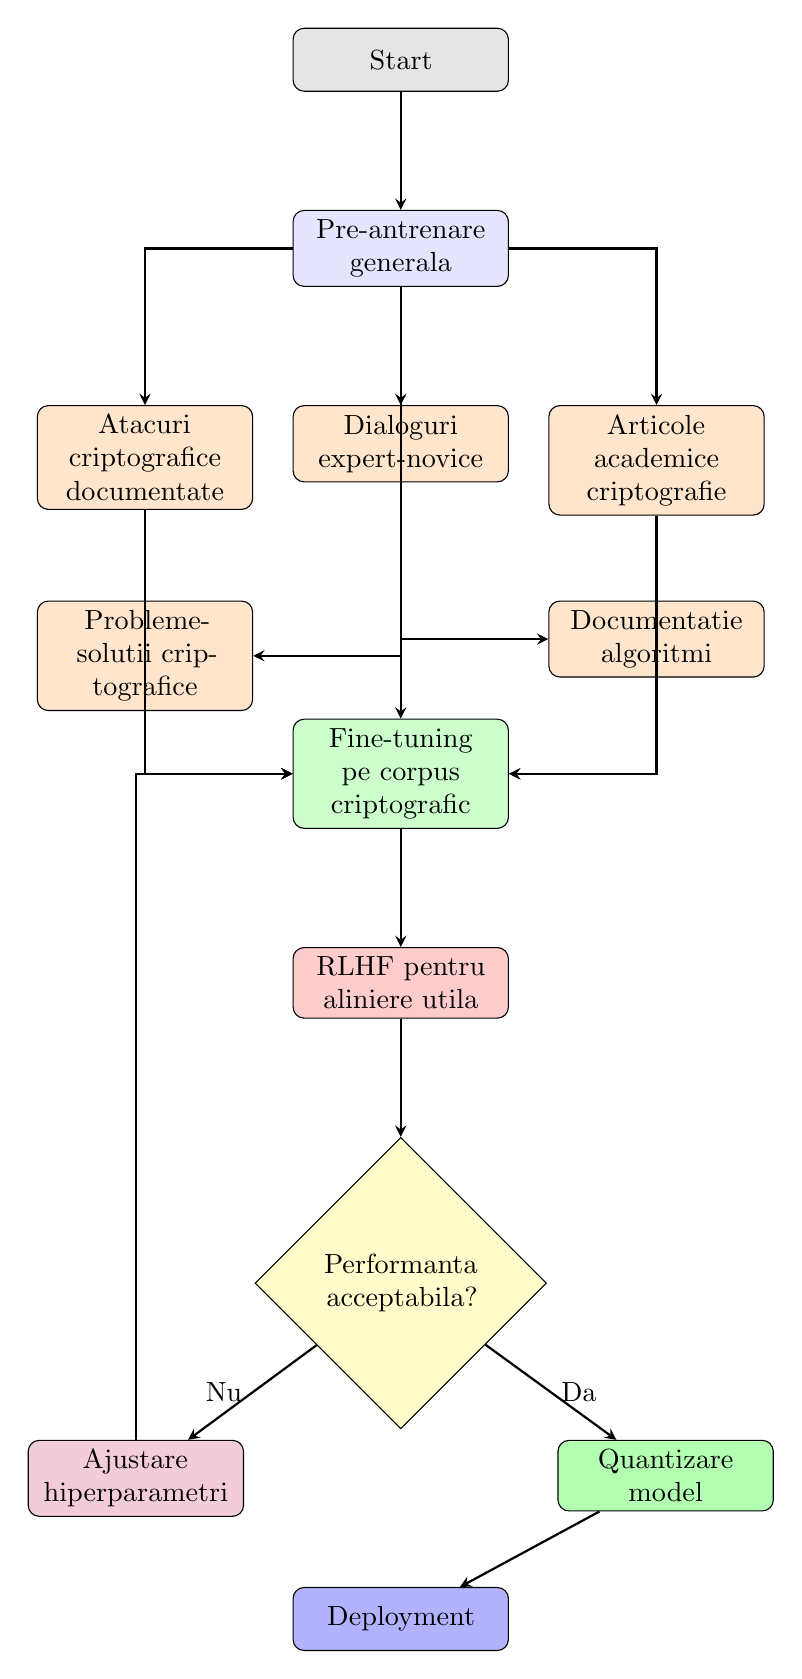
\begin{tikzpicture}[
    node distance=1.5cm,
    block/.style={rectangle, draw, fill=blue!20, text width=2.5cm, text centered, minimum height=0.8cm, rounded corners},
    decision/.style={diamond, draw, fill=yellow!20, text width=2.5cm, text centered, minimum height=1cm},
    arrow/.style={thick,->,>=stealth}
    ]
    
    
    \node[block, fill=gray!20] (start) {Start};
    
    
    \node[block, fill=blue!10] (pretraining) [below=of start] {Pre-antrenare generala};
    
    
    \node[block, fill=orange!20] (data1) [below left=1.5cm and 0.5cm of pretraining] {Atacuri criptografice documentate};
    \node[block, fill=orange!20] (data2) [below=of pretraining] {Dialoguri expert-novice};
    \node[block, fill=orange!20] (data3) [below right=1.5cm and 0.5cm of pretraining] {Articole academice criptografie};
    \node[block, fill=orange!20] (data4) [below left=1.5cm and 0.5cm of data2] {Probleme-solutii criptografice};
    \node[block, fill=orange!20] (data5) [below right=1.5cm and 0.5cm of data2] {Documentatie algoritmi};
    
    
    \node[block, fill=green!20] (finetuning) [below=3cm of data2] {Fine-tuning pe corpus criptografic};
    
    
    \node[block, fill=red!20] (rlhf) [below=of finetuning] {RLHF pentru aliniere utila};
    
    
    \node[decision] (eval) [below=of rlhf] {Performanta acceptabila?};
    
    
    \node[block, fill=purple!20] (adjust) [below left=of eval] {Ajustare hiperparametri};
    \node[block, fill=green!30] (quantize) [below right=of eval] {Quantizare model};
    
    
    \node[block, fill=blue!30] (deploy) [below=2cm of eval] {Deployment};
    
    
    \draw[arrow] (start) -- (pretraining);
    \draw[arrow] (pretraining) -| (data1);
    \draw[arrow] (pretraining) -- (data2);
    \draw[arrow] (pretraining) -| (data3);
    \draw[arrow] (pretraining) |- (data4);
    \draw[arrow] (pretraining) |- (data5);
    
    \draw[arrow] (data1) |- (finetuning);
    \draw[arrow] (data2) -- (finetuning);
    \draw[arrow] (data3) |- (finetuning);
    \draw[arrow] (data4) |- (finetuning);
    \draw[arrow] (data5) |- (finetuning);
    
    \draw[arrow] (finetuning) -- (rlhf);
    \draw[arrow] (rlhf) -- (eval);
    \draw[arrow] (eval) -- node[left] {Nu} (adjust);
    \draw[arrow] (eval) -- node[right] {Da} (quantize);
    \draw[arrow] (adjust) |- (finetuning);
    \draw[arrow] (quantize) -- (deploy);
    
  \end{tikzpicture}
  \caption{Strategia de antrenare pentru LLM specializat}
  \label{fig:antrenare}
\end{figure}

\subsection{Setul de Date pentru Antrenare}
\begin{itemize}
  \item \textbf{Corpus General}: Modele pre-antrenate (ex. Llama 3, Mistral, etc.)
  \item \textbf{Corpus Specializat}:
  \begin{itemize}
    \item Articole academice din domeniul criptografiei
    \item Documentatie pentru algoritmi criptografici
    \item Perechi problema-solutie din criptografie
    \item Exemple de atacuri criptografice si rezolvarile lor
    \item Dialoguri expert-novice in domeniul criptografiei
    \item Manuale si carti de specialitate in format digital
  \end{itemize}
\end{itemize}

\subsection{Fine-tuning si RLHF}
\begin{itemize}
  \item \textbf{Fine-tuning Supervizat}: Pe corpus specializat criptografic
  \item \textbf{RLHF (Reinforcement Learning from Human Feedback)}: Pentru aliniere si utilitate
  \item \textbf{Prompting Specializat}: Tehnici de few-shot si chain-of-thought pentru probleme complexe
\end{itemize}

\section{Motorul de Analiza Criptografica}

\subsection{Componente}
\begin{itemize}
  \item \textbf{Detector de Algoritm}: Model de clasificare pentru identificarea tipului de criptare
  \item \textbf{Analizor Frecvente}: Pentru criptografie clasica
  \item \textbf{Module Specializate}: Pentru fiecare algoritm major (AES, RSA, DES, etc.)
  \item \textbf{Executor de Atacuri}: Implementarea automatizata a atacurilor cunoscute
\end{itemize}

\subsection{Fluxuri de Lucru}

  

\subsection{Detector de Algoritm}
Detectorul de algoritm va folosi o abordare hibrida:

\begin{enumerate}
  \item \textbf{Analiza Structurala}:
  \begin{itemize}
    \item Verificarea lungimii output-ului
    \item Identificarea pattern-urilor specifice (ex. padding)
    \item Verificarea entropiei
  \end{itemize}

  \item \textbf{Clasificare ML}:
  \begin{itemize}
    \item Model CNN + LSTM pentru identificarea algoritmilor din text criptat
    \item Features extrase din distributii statistice
  \end{itemize}

  \item \textbf{Euristica Bazata pe Reguli}:
  \begin{itemize}
    \item Reguli predefinite pentru algoritmi cunoscuti
    \item Verificari pentru semnaturi specifice
  \end{itemize}
\end{enumerate}

\begin{lstlisting}[language=Python, caption={Exemplu conceptual pentru detectorul de algoritm}]
# Exemplu conceptual pentru detectorul de algoritm
class CipherDetector:
    def __init__(self):
        self.statistical_analyzer = StatisticalAnalyzer()
        self.ml_classifier = load_model("cipher_classifier.h5")
        self.rule_engine = RuleBasedDetector()
        
    def detect(self, ciphertext, additional_info=None):
        # Analiza statistica
        stats_features = self.statistical_analyzer.extract_features(ciphertext)
        
        # Clasificare ML
        ml_predictions = self.ml_classifier.predict(self.preprocess(ciphertext))
        
        # Verificare euristici
        rule_candidates = self.rule_engine.apply_rules(ciphertext, additional_info)
        
        # Fuziune rezultate
        final_candidates = self.fusion_algorithm(stats_features, ml_predictions, rule_candidates)
        
        return sorted(final_candidates, key=lambda x: x['confidence'], reverse=True)
\end{lstlisting}

\section{Modulul de Teorie a Numerelor}

\subsection{Functionalitati}
\begin{itemize}
  \item \textbf{Teste de Primalitate}:
  \begin{itemize}
    \item Miller-Rabin
    \item AKS (Agrawal-Kayal-Saxena)
    \item Lucas-Lehmer (pentru numere Mersenne)
  \end{itemize}

  \item \textbf{Factorizare}:
  \begin{itemize}
    \item Trial division
    \item Metoda Pollard Rho
    \item Quadratic Sieve
    \item Number Field Sieve (pentru numere mari)
  \end{itemize}

  \item \textbf{Operatii Speciale}:
  \begin{itemize}
    \item Calculul logaritmului discret
    \item Operatii pe curbe eliptice
    \item Generare numere prime de dimensiuni specifice
  \end{itemize}
\end{itemize}

\subsection{Integrare cu Baze de Date Externe}
\begin{itemize}
  \item Interogare automata FactorDB
  \item Cache local pentru rezultate frecvente
  \item Sincronizare periodica cu baze de date publice
\end{itemize}

\section{Modulul de Analiza Parole}

\subsection{Metrici de Securitate}
\begin{itemize}
  \item \textbf{Entropie}: Calculata pe baza seturilor de caractere si lungimii
  \item \textbf{Rezistenta la Atacuri}: Estimare timp pentru diferite tipuri de atacuri
  \item \textbf{Verificare in Baze de Date}: CrackStation, HaveIBeenPwned
  \item \textbf{Analiza Structurala}: Identificare pattern-uri comune, substitutii predictibile
\end{itemize}

\subsection{Vizualizare si Recomandari}

\section{Implementarea Algoritmilor Post-Quantum}

\subsection{Algoritmi Selectati}
\begin{itemize}
  \item \textbf{Criptare Asimetrica}:
  \begin{itemize}
    \item Kyber (CRYSTALS-Kyber): Selectat de NIST ca standard
    \item NTRU: Alternativa matura si studiata
  \end{itemize}
  \item \textbf{Semnaturi Digitale}:
  \begin{itemize}
    \item Dilithium (CRYSTALS-Dilithium): Standard NIST
    \item FALCON: Pentru aplicatii cu semnaturi compacte
  \end{itemize}
  \item \textbf{Schimb de Chei}:
  \begin{itemize}
    \item SIKE: Supersingular Isogeny Key Encapsulation
  \end{itemize}
\end{itemize}

\subsection{Implementare si Integrare}
\begin{itemize}
  \item Utilizarea bibliotecii liboqs ca baza
  \item Wrapper-uri Python pentru acces simplificat
  \item Integrare in fluxurile de lucru standard
  \item Interfete compatibile cu algoritmi clasici pentru tranzitie usoara
\end{itemize}

\chapter{Securizarea Sistemului}

\section{Autentificare si Autorizare}
\begin{itemize}
  \item \textbf{JWT} pentru tokenuri de acces
  \item \textbf{OAuth2} pentru autorizare
  \item \textbf{Rate limiting} pentru prevenirea abuzului
  \item \textbf{RBAC} (Role-Based Access Control) pentru permisiuni granulare
\end{itemize}

\section{Securitatea Comunicatiilor}
\begin{itemize}
  \item \textbf{TLS 1.3} pentru toate comunicatiile externe
  \item \textbf{Mutual TLS} pentru comunicatii intre microservicii
  \item \textbf{Perfect Forward Secrecy} pentru protectie pe termen lung
\end{itemize}

\section{Securitatea Datelor}
\begin{itemize}
  \item \textbf{Criptare la repaus} pentru toate datele sensibile
  \item \textbf{Tokenizare} pentru informatii de identificare personala
  \item \textbf{Anonimizare} a datelor utilizate pentru antrenare
\end{itemize}

\chapter{Deployment si Scalabilitate}

\section{Arhitectura Docker}

\section{Implementare Kubernetes}
\begin{itemize}
  \item \textbf{Namespace Dedicat}: Izolare completa a resurselor
  \item \textbf{Deployment} pentru fiecare serviciu cu strategie de rolling update
  \item \textbf{HorizontalPodAutoscaler} pentru scalare bazata pe utilizare
  \item \textbf{Ingress} pentru routare externa si TLS
  \item \textbf{Helm Charts} pentru deployments reproductibile
  \item \textbf{Secrets Management} cu Kubernetes Secrets sau HashiCorp Vault
\end{itemize}

\section{Monitoring si Logging}
\begin{itemize}
  \item \textbf{Prometheus} pentru colectarea metricilor
  \item \textbf{Grafana} pentru dashboards si vizualizare
  \item \textbf{ELK Stack} (Elasticsearch, Logstash, Kibana) pentru logging centralizat
  \item \textbf{Alerting} pentru notificari proactive in caz de probleme
\end{itemize}

\chapter{Fluxuri de Lucru Detaliate}

\section{Conversatie cu LLM pentru Rezolvarea Problemelor}
\begin{enumerate}
  \item \textbf{Initiere}: Utilizatorul descrie o problema criptografica
  \item \textbf{Intelegere}: LLM proceseaza si extrage componentele cheie
  \item \textbf{Clarificare}: LLM cere detalii suplimentare daca este necesar
  \item \textbf{Rezolvare}: LLM genereaza solutia pas cu pas
  \item \textbf{Explicare}: LLM ofera detalii despre abordarea folosita
  \item \textbf{Feedback}: Utilizatorul poate cere clarificari sau detalii suplimentare
\end{enumerate}

\begin{tcolorbox}[colback=infobox, colframe=blue!50!black, title=Exemplu Conversatie]
\begin{verbatim}
Utilizator: Cum pot decripta acest text "Uifsf jt b tfdsfu nfttbhf"?

LLM: Acest text pare sa fie criptat cu Caesar Cipher (sau ROT). 
Voi incerca diferite chei:

Cu ROT-1: "There is a secret message"
Aceasta varianta are sens in limba engleza, deci probabil este corecta. 
Cifrul Caesar inlocuieste 
fiecare litera cu litera aflata la o anumita pozitie fixa in alfabet. 
In acest caz, fiecare litera a fost inlocuita cu urmatoarea 
litera din alfabet (ROT-1).
Doriti sa aflati mai multe despre cifrul Caesar sau cum sa detectati 
acest tip de criptare?
\end{verbatim}
\end{tcolorbox}

\section{Analiza Mesajului Criptat}
\begin{enumerate}
  \item \textbf{Incarcare}: Utilizatorul trimite textul criptat
  \item \textbf{Detectare}: Sistemul detecteaza algoritmul de criptare probabil
  \item \textbf{Analiza}: Se executa analize statistice si pattern matching
  \item \textbf{Atac}: Se incearca metode de atac pentru algoritmul detectat
  \item \textbf{Raportare}: Se returneaza rezultatele si explicatiile
\end{enumerate}

\section{Lucrul cu Algoritmi Post-Quantum}
\begin{enumerate}
  \item \textbf{Selectie}: Utilizatorul alege tipul de algoritm post-quantum
  \item \textbf{Configurare}: Se seteaza parametrii specifici
  \item \textbf{Generare}: Se genereaza cheile criptografice
  \item \textbf{Operatii}: Se efectueaza operatiuni (criptare, semnare, etc.)
  \item \textbf{Analiza}: Se ofera statistici si comparatii cu algoritmi clasici
\end{enumerate}

\begin{lstlisting}[language=Python, caption={Exemplu de utilizare pentru CRYSTALS-Kyber}]
# Exemplu simplificat de integrare Kyber in aplicatie
from pqcrypto import kyber

# Generare chei
public_key, secret_key = kyber.keygen()

# Criptare mesaj
ciphertext, shared_secret_enc = kyber.encrypt(public_key, message)

# Decriptare mesaj
shared_secret_dec = kyber.decrypt(secret_key, ciphertext)

# Verificare
assert shared_secret_enc == shared_secret_dec
\end{lstlisting}

\chapter{Antrenarea Modelelor ML/DL}

\section{Model pentru Detectarea Algoritmului de Criptare}

\subsection{Procesul de Antrenare}
\begin{enumerate}
  \item \textbf{Pregatirea Datelor}:
  \begin{itemize}
    \item Generarea datelor pentru multiple algoritmi (AES, DES, RSA, etc.)
    \item Variatii in chei, moduri de operare, padding
    \item Augmentarea datelor pentru robustete
  \end{itemize}

  \item \textbf{Arhitectura Modelului}:
  \begin{itemize}
    \item CNN pentru extragerea pattern-urilor locale
    \item BiLSTM pentru capturarea dependentelor secventiale
    \item Fully Connected layers pentru clasificare
  \end{itemize}

  \item \textbf{Strategia de Antrenare}:
  \begin{itemize}
    \item Transfer learning de la modele antrenate pe clasificare de text
    \item Fine-tuning specific pentru date criptografice
    \item Validation cruce pentru evitarea overfitting
  \end{itemize}
\end{enumerate}

\subsection{Evaluare si Optimizare}
\begin{itemize}
  \item Matrice de confuzie pentru intelegerea erorilor
  \item Raport de clasificare (precision, recall, F1)
  \item Evaluare pe date din lumea reala
  \item Analiza cazurilor de esec pentru imbunatatire
\end{itemize}

\section{Antrenare LLM Specializat}

\subsection{Procesul de Fine-tuning}
\begin{enumerate}
  \item \textbf{Selectia Modelului de Baza}:
  \begin{itemize}
    \item Utilizarea unui model pre-antrenat (ex. Llama 3-8B)
    \item Adaptarea arhitecturii pentru context specializat
  \end{itemize}

  \item \textbf{Pregatirea Datelor}:
  \begin{itemize}
    \item Colectarea si curatarea corpusului criptografic
    \item Structurarea in formatul instruction-response
    \item Augmentarea cu date sintetice
  \end{itemize}

  \item \textbf{Fine-tuning}:
  \begin{itemize}
    \item LoRA (Low-Rank Adaptation) pentru eficienta
    \item QLoRA pentru training pe hardware accesibil
    \item Strategii de optimizare a hiperparametrilor
  \end{itemize}
\end{enumerate}

\subsection{RLHF (Reinforcement Learning from Human Feedback)}
\begin{enumerate}
  \item \textbf{Colectarea Preferintelor}:
  \begin{itemize}
    \item Evaluari de experti in domeniul criptografiei
    \item Comparatii intre raspunsuri alternative
  \end{itemize}

  \item \textbf{Antrenarea Modelului de Recompensa}:
  \begin{itemize}
    \item Model care prezice preferintele umane
    \item Calibrare pentru evitarea biasurilor
  \end{itemize}

  \item \textbf{Optimizare prin PPO}:
  \begin{itemize}
    \item Fine-tuning folosind Proximal Policy Optimization
    \item Balansare intre maximizarea recompensei si evitarea devierilor
  \end{itemize}
\end{enumerate}

\chapter{Planificarea Proiectului}

\section{Etape si Termene}

% \begin{figure}[h]
%   \centering
%   \begin{tikzpicture}[x=0.037cm, y=0.4cm, scale=0.8, transform shape]
%     % Elimină grid-ul
    
%     % Axa temporală simplificată
%     \draw[->] (0, 8) -- (1200, 8);
%     \foreach \x in {0, 300, 600, 900, 1200}
%       \draw (\x, 8) -- (\x, 7.8) node[above] {\footnotesize \x};
    
%     % Etichete pentru etape - codificate cu litere
%     \node[anchor=east, font=\footnotesize] at (0, 7) {A};
%     \node[anchor=east, font=\footnotesize] at (0, 6) {B};
%     \node[anchor=east, font=\footnotesize] at (0, 5) {C};
%     \node[anchor=east, font=\footnotesize] at (0, 4) {D};
%     \node[anchor=east, font=\footnotesize] at (0, 3) {E};
%     \node[anchor=east, font=\footnotesize] at (0, 2) {F};
    
%     % Task-uri grupate pe culori, cu coduri numerice simple
%     % Analiză și Design (A)
%     \filldraw[fill=blue!20, draw=blue!50] (0, 6.8) rectangle (150, 7.2) node[midway, font=\tiny] {1};
%     \filldraw[fill=blue!20, draw=blue!50] (150, 6.8) rectangle (250, 7.2) node[midway, font=\tiny] {2};
%     \filldraw[fill=blue!20, draw=blue!50] (250, 6.8) rectangle (350, 7.2) node[midway, font=\tiny] {3};
    
%     % Backend (B)
%     \filldraw[fill=green!20, draw=green!50] (250, 5.8) rectangle (400, 6.2) node[midway, font=\tiny] {1};
%     \filldraw[fill=green!20, draw=green!50] (400, 5.8) rectangle (500, 6.2) node[midway, font=\tiny] {2};
%     \filldraw[fill=green!20, draw=green!50] (400, 5.3) rectangle (550, 5.7) node[midway, font=\tiny] {3};
%     \filldraw[fill=green!20, draw=green!50] (450, 4.8) rectangle (550, 5.2) node[midway, font=\tiny] {4};
%     \filldraw[fill=green!20, draw=green!50] (550, 5.8) rectangle (700, 6.2) node[midway, font=\tiny] {5};
    
%     % LLM și AI (C)
%     \filldraw[fill=orange!20, draw=orange!50] (300, 4.8) rectangle (450, 5.2) node[midway, font=\tiny] {1};
%     \filldraw[fill=orange!20, draw=orange!50] (450, 4.8) rectangle (600, 5.2) node[midway, font=\tiny] {2};
%     \filldraw[fill=orange!20, draw=orange!50] (400, 4.3) rectangle (500, 4.7) node[midway, font=\tiny] {3};
%     \filldraw[fill=orange!20, draw=orange!50] (600, 4.8) rectangle (700, 5.2) node[midway, font=\tiny] {4};
    
%     % Frontend (D)
%     \filldraw[fill=cyan!20, draw=cyan!50] (450, 3.8) rectangle (550, 4.2) node[midway, font=\tiny] {1};
%     \filldraw[fill=cyan!20, draw=cyan!50] (500, 3.3) rectangle (600, 3.7) node[midway, font=\tiny] {2};
%     \filldraw[fill=cyan!20, draw=cyan!50] (500, 3.8) rectangle (650, 4.2) node[midway, font=\tiny] {3};
    
%     % Integrare (E)
%     \filldraw[fill=purple!20, draw=purple!50] (650, 2.8) rectangle (750, 3.2) node[midway, font=\tiny] {1};
%     \filldraw[fill=purple!20, draw=purple!50] (750, 2.8) rectangle (850, 3.2) node[midway, font=\tiny] {2};
%     \filldraw[fill=purple!20, draw=purple!50] (850, 2.8) rectangle (950, 3.2) node[midway, font=\tiny] {3};
    
%     % Finalizare (F)
%     \filldraw[fill=red!20, draw=red!50] (500, 1.8) rectangle (1100, 2.2) node[midway, font=\tiny] {1};
%     \filldraw[fill=red!20, draw=red!50] (1000, 1.3) rectangle (1100, 1.7) node[midway, font=\tiny] {2};
%     \filldraw[fill=red!20, draw=red!50] (1100, 1.8) rectangle (1200, 2.2) node[midway, font=\tiny] {3};
    
%   \end{tikzpicture}
  
%   \vspace{0.2cm}
%   {\footnotesize
%   \begin{tabular}{ll|ll|ll}
%     \textbf{Etape} & & \multicolumn{4}{l}{\textbf{Sarcini}} \\
%     \hline
%     A Analiză & & A1 Cercetare & B3 Teorie numere & D1 API \\
%     B Backend & & A2 Cerințe & B4 Parole & D2 CLI \\
%     C ML/AI & & A3 Arhitectură & B5 Post-quantum & D3 Web \\
%     D Frontend & & B1 Framework & C1 Date & E1 Integrare \\
%     E Testare & & B2 Criptografie & C2 LLM & E2 Testare \\
%     F Finalizare & & & C3 Detector & E3 Optimizare \\
%     & & & C4 RLHF & F1-F3 Documentație \\
%   \end{tabular}
%   }
%   \caption{Planificare proiect}
%   \label{fig:gantt-simplificat}
% \end{figure}

\section{Estimare Efort si Resurse}

\begin{table}[h]

\centering
\begin{tabularx}{\textwidth}{|X|c|c|X|}
\toprule
\textbf{Componenta} & \textbf{Efort Estimat (ore)} & \textbf{Nivel Complexitate} & \textbf{Resurse Necesare} \\
\midrule
Arhitectura si design & 80-120 & Mediu & Documentatie, cercetare \\
Motor LLM (fine-tuning) & 150-200 & Inalt & GPU performant, date antrenare \\
Motor criptografic & 100-150 & Mediu-Inalt & Biblioteci criptografice \\
Modul teorie numere & 80-100 & Mediu & Biblioteci matematice \\
Analiza parole & 60-80 & Mediu & Baze de date, biblioteci statistice \\
Algoritmi post-quantum & 100-120 & Inalt & Documentatie specializata \\
Frontend si API & 100-120 & Mediu & Biblioteci UI, framework web \\
Integrare si testare & 80-100 & Mediu & Framework-uri de testare \\
Documentatie & 70-100 & Mediu & Materiale referinta \\
\midrule
\textbf{Total} & \textbf{820-1090} & & \\
\bottomrule
\end{tabularx}
\caption{Estimare efort si resurse}
\label{tab:efort}
\end{table}

\section{Managementul Riscurilor}
\begin{table}[h]
\centering
\begin{tabularx}{\textwidth}{|X|c|c|X|}
\toprule
\textbf{Risc} & \textbf{Probabilitate} & \textbf{Impact} & \textbf{Strategii de Mitigare} \\
\midrule
Complexitate tehnica neprevazuta & Medie & Inalt & Prototipare rapida, cercetare aprofundata \\
Limitari hardware pentru antrenare LLM & Inalta & Mediu & Utilizare modele mai mici, tehnici eficiente (QLoRA) \\
Integrare dificila a componentelor & Medie & Mediu & Dezvoltare bazata pe API, testare continua \\
Securitatea sistemului compromisa & Scazuta & Foarte Inalt & Audit de securitate, testare penetrare \\
Timelines nerealist & Medie & Inalt & Buffer in planificare, prioritizare caracteristici \\
\bottomrule
\end{tabularx}
\caption{Managementul riscurilor}
\label{tab:riscuri}
\end{table}

\chapter{Consideratii Finale}

\section{Contributii Academice}
Proiectul contribuie in mai multe directii:
\begin{itemize}
  \item Integrarea tehnicilor de ML/DL in analiza criptografica
  \item Arhitectura hibrida pentru instrumente criptografice
  \item Implementarea practica a algoritmilor post-quantum
  \item Framework conversational pentru probleme criptografice
\end{itemize}

\section{Potentiale Extensii}
\begin{itemize}
  \item Suport pentru noi algoritmi criptografici
  \item Integrarea cu sisteme de PKI (Public Key Infrastructure)
  \item Dezvoltarea unui framework pentru competitii CTF
  \item Modul de analiza forensica pentru malware criptat
  \item Integrare cu sisteme de blockchain
\end{itemize}

\section{Limitari si Provocari}
\begin{itemize}
  \item Performanta inferentei LLM pe hardware limitat
  \item Actualizarea constanta a bazelor de date
  \item Mentinerea la curent cu evolutiile in criptanaliza
  \item Consideratii etice pentru unelte de atac criptografic
\end{itemize}

\chapter{Referinte si Resurse Utile}

                        \section{Referințe și Resurse}

\subsection{Cărți și Manuale}
\begin{enumerate}
    \item Ferguson, N., Schneier, B., \& Kohno, T. (2022). \textit{Cryptography Engineering: Design Principles and Practical Applications}. Wiley.
    \item Paar, C., \& Pelzl, J. (2021). \textit{Understanding Cryptography: A Textbook for Students and Practitioners}. Springer.
    \item Boneh, D., \& Shoup, V. (2023). \textit{A Graduate Course in Applied Cryptography}. [Online] Disponibil la: \url{https://toc.cryptobook.us/}
    \item Jurafsky, D., \& Martin, J. H. (2023). \textit{Speech and Language Processing}. [Online] Disponibil la: \url{https://web.stanford.edu/~jurafsky/slp3/}
    \item Bernstein, D. J., \& Lange, T. (2021). \textit{Post-Quantum Cryptography}. Springer.
\end{enumerate}

\subsection{Articole Academice}
\begin{enumerate}
    \item Alagic, G., et al. (2023). "Status Report on the Third Round of the NIST Post-Quantum Cryptography Standardization Process." NIST.
    \item Devlin, J., Chang, M. W., Lee, K., \& Toutanova, K. (2019). "BERT: Pre-training of Deep Bidirectional Transformers for Language Understanding." NAACL.
    \item Ouyang, L., et al. (2022). "Training language models to follow instructions with human feedback." NeurIPS.
    \item Bernstein, D. J. (2023). "Comparing proofs of security for lattice-based encryption." \textit{Journal of Cryptology}.
    \item Fouque, P. A., et al. (2022). "FALCON: Fast-Fourier Lattice-based Compact Signatures over NTRU." NIST PQC.
\end{enumerate}

\subsection{Documentație Tehnică și Standarde}
\begin{enumerate}
    \item NIST (2023). \textit{FIPS 197: Advanced Encryption Standard (AES).}
    \item NIST (2022). \textit{SP 800-38A: Recommendation for Block Cipher Modes of Operation.}
    \item IETF (2024). \textit{RFC 8446: The Transport Layer Security (TLS) Protocol Version 1.3.}
    \item ISO/IEC (2022). \textit{ISO/IEC 29192: Information technology — Security techniques — Lightweight cryptography.}
    \item NIST (2023). \textit{SP 800-208: Recommendation for Stateful Hash-Based Signature Schemes.}
\end{enumerate}

\subsection{Resurse Online și Tutoriale}
\begin{enumerate}
    \item \textit{CryptoPals Crypto Challenges}. [Online] Disponibil la: \url{https://cryptopals.com/}
    \item \textit{Cryptography I \& II}. Coursera (Stanford University). [Online]
    \item \textit{Post-Quantum Cryptography}. NIST. [Online] Disponibil la: \url{https://csrc.nist.gov/projects/post-quantum-cryptography}
    \item \textit{The Illustrated Transformer}. [Online] Disponibil la: \url{http://jalammar.github.io/illustrated-transformer/}
    \item \textit{Real-World Cryptography}. [Online] Disponibil la: \url{https://www.manning.com/books/real-world-cryptography}
\end{enumerate}

\subsection{Biblioteci și Framework-uri}
\begin{enumerate}
    \item OpenSSL Documentation. [Online] Disponibil la: \url{https://www.openssl.org/docs/}
    \item PyTorch Documentation. [Online] Disponibil la: \url{https://pytorch.org/docs/stable/index.html}
    \item Hugging Face Transformers Documentation. [Online] Disponibil la: \url{https://huggingface.co/docs/transformers/}
    \item FastAPI Documentation. [Online] Disponibil la: \url{https://fastapi.tiangolo.com/}
    \item liboqs: C library for quantum-resistant cryptographic algorithms. [Online] Disponibil la: \url{https://github.com/open-quantum-safe/liboqs}
\end{enumerate}

\subsection{Instrumente și Resurse Relevante}
\begin{enumerate}
    \item \textit{dcode.fr} - Cryptography tools collection. [Online] Disponibil la: \url{https://www.dcode.fr/}
    \item \textit{CyberChef} - Web app for encryption, encoding, compression and data analysis. [Online] Disponibil la: \url{https://gchq.github.io/CyberChef/}
    \item \textit{FactorDB} - Database of large integer factorizations. [Online] Disponibil la: \url{http://factordb.com/}
    \item \textit{RSACTFTool} - RSA attack tool. [Online] Disponibil la: \url{https://github.com/RsaCtfTool/RsaCtfTool}
    \item \textit{Have I Been Pwned} - Compromised password checking service. [Online] Disponibil la: \url{https://haveibeenpwned.com/}
\end{enumerate}


\chapter*{Concluzii}
\addcontentsline{toc}{chapter}{Concluzii}

Acest proiect propune o abordare integrata si moderna pentru analiza criptografica, combinand tehnici traditionale cu inteligenta artificiala si machine learning. Prin integrarea unui motor LLM specializat, utilizatorii vor putea interactiona natural cu sistemul pentru a rezolva probleme criptografice complexe, analizand criptograme, evaluand securitatea parolelor si explorand algoritmi post-quantum.

Implementarea foloseste tehnologii de varf precum Docker pentru containerizare, FastAPI pentru backend, PyTorch pentru componente de ML/DL, si implementari native C/C++ pentru algoritmi criptografici performanti. Arhitectura modulara permite extensibilitate si scalabilitate, iar abordarea bazata pe microservicii faciliteaza dezvoltarea si testarea independenta a componentelor.

Cu un timp estimat de implementare de 800-1000 de ore, proiectul este fezabil pentru o lucrare de licenta ambitioasa, oferind atat valoare academica prin cercetarea aplicata, cat si valoare practica prin crearea unui instrument util pentru educatie si cercetare in domeniul securitatii informatice.

Adoptarea unui model de dezvoltare iterativ, cu focus initial pe functionalitatile de baza si extindere graduala a capacitatilor, va permite gestionarea eficienta a complexitatii si livrarea unui produs functional in limitele de timp disponibile.

\end{document}